\documentclass[journal,onecolumn]{IEEEtran}


\ifCLASSINFOpdf
  
\else
  
\fi

\hyphenation{op-tical net-works semi-conduc-tor}
\usepackage{booktabs}
\usepackage{array}
\usepackage{multirow}
\usepackage{pgfplotstable}
\usepackage{colortbl}
\usepackage{xcolor}
\usepackage{graphicx}
\usepackage{pgfplots}
\usepackage{placeins}
\pgfplotsset{compat=1.18}
\renewcommand{\arraystretch}{1.15}

%\newcommand{\strategyalg}[1]{% \StrBefore{#1}{::}[\algtemp]% \algtemp% } \newcommand{\strategyheur}[1]{% \StrBehind{#1}%{::}[\heurtemp]% \heurtemp% }
\usepackage{xstring}

\begin{document}

\title{Design and Implementation of an Intelligent Agent for Competitive Dominoes Integrating A*, Minimax and Distance-Based Heuristics}


\author{Jazmin Dajerly Moreno Galindo, Sebastian David Lizarazo Duarte\\ 
Universidad Pedagógica y Tecnológica de Colombia \\ 
Sogamoso, Colombia \\ 
jazmin.moreno01@uptc.edu.co\\
sebastian.lizarazo03@uptc.edu.co}


\maketitle

\begin{abstract}
Este informe presenta el desarrollo de un agente de inteligencia artificial (AI) para el juego de domino implementando los algoritmos Minimax y alfa-beta. El proyecto permite simular partidas entre dos agentes inteligentes, evaluando su desempeño con cada una de las heurísticas definidas: lineal, Manhattan y euclidiana, analizando la eficiencia de cada uno en la toma de decisiones y mostrando el desempeño de cada uno de los algoritmos. Los resultados muestran que ambos obtuvieron desempeños similares para las victorias, pero la poda alfa-beta reduce ampliamente el número de nodos explorados y tiempo de decisión reduciendo asi el costo computacional 
\end{abstract}

\begin{IEEEkeywords}
AI, Minimax, Alfa-Beta, Heuristicas, Manhattan, Euclidiana, costo computacional
\end{IEEEkeywords}

\IEEEpeerreviewmaketitle



\section{Introduction}
Introduction goes here

\section{Related Work}
\subsection{Algoritmo A* en videojuegos}
En \cite{liu2023research} el autor implementa una aplicación del algoritmo \textit{A*} en el campo de los videojuegos, enfatizando su papel como técnica heurística para la búsqueda de rutas en entornos discretos. El autor utiliza la función \textit{f(n) = g(n) + h(n)}, donde \textit{g(n)} es el coste acumulado desde el nodo inicial y \textit{h(n)} la estimación del coste restante, y muestra cómo esta combinación permite priorizar estados con mayor probabilidad de conducir a soluciones eficientes.\\
Dicho trabajo destaca que la implementación de heurísticas como la \textbf{distancia Manhattan} condiciona el patrón de expansión y eficiencia. Para el caso de la heurística ya mencionada, esta se caracteriza por su efectividad en mallas de conectividad ortogonal, mientras que aproximaciones euclidianas se suelen emplear cuando se permite movimiento en diagonal. \cite{liu2023research} demuestra que una heurística bien diseñada reduce la expansión innecesaria de nodos y, por ende, mejora el rendimiento sin sacrificar efectividad.\\
Las conclusiones presentes en \cite{liu2023research} son transferibles al problema de evaluación de estados y selección de jugadas. En ambos casos, el algoritmo debe discriminar entre alternativas plausibles y priorizar opciones prometedoras; por ello, la metodología de combinar coste acumulado y estimación heurística ofrece una base conceptual sólida para diseñar criterios de decisión en agentes de juego.\\
Para el prototipo de dominó construido en el presente proyecto, se tuvieron en cuenta 2 lecciones prácticas de \cite{liu2023research}:\\
\begin{itemize}
    \item 1. \textit{A*} provee una base robusta para formular criterios cuando se puede definir un espacio de estados y una heurística admisible.\\
    \item 2. Las optimizaciones de estructuras de datos y las adaptaciones en tiempo real son necesarias para garantizar respuestas con latencia aceptable en entornos interactivos.
\end{itemize}
\subsection{Algorirmo Minimax y Alpha-Beta pruning}
Shevtekar y Kulkarni presentan en \cite{kulkarni2022minimax} una revisión práctica de los algoritmos de búsqueda adversarial aplicados a juegos de dos jugadores, describiendo la implementación de \textbf{Minimax} optimizada mediante \textbf{Alpha-Beta pruning}, además de variantes como \textbf{NegaScout}. Muestran cómo estas técnicas permiten evitar la exploración de subárboles que no pueden influir en la decisión final.\\
El trabajo reafirma a \textbf{Minimax} como el método estándar para seleccionar movimientos ideales en juegos de suma cero asumiendo adversarios óptimos. La optimización por \textbf{Alpha-Beta pruning} reduce drásticamente el número de nodos evaluados sin alterar el resultado que devolvería Minimax, permitiendo búsquedas más profundas en el mismo rango de tiempo.


\section{Materials and Methods}
Para el desarrollo del agente de inteligencia artificial es necesario establecer las herramientas, algoritmos y reglas del juego que se implementarán y tendrán en cuenta. 

Inicialmente se definió el concepto de agente de IA, a continuación se dio contexto del juego de domino, ya que a través de sus reglas se establece la forma en que el agente interactúa con el sistema y toma decisiones durante la partida y finalmente se presentan los algoritmos implementados para el desarrollo del agente


\subsection{ AI agents}
Un agente de inteligencia artificial es un sistema de software que usa técnicas de IA para alcanzar objetivos y completar tareas de forma autónoma, para alcanzarlo, percibe su entorno, tienen patrones de razonamiento, planificación y memoria. Estos sistemas son capaces de tomar decisiones, aprender de la experiencia, solucionar problemas  y adaptarse, reduciendo la intervención humana \cite{akerkar}

\subsection{ Domino }
El juego implementado corresponde a una versión del dominó para dos jugadores, el juego está compuesto por 28 fichas. El objetivo es ser el primer jugador en quedarse sin fichas o tener la menor cantidad de puntos cuando no se tengan más movimientos válidos \cite{RuibalDomino2015}

Cada jugador inicia la partida con 7 fichas seleccionadas aleatoriamente. Las fichas restantes no haran parte del juego

El juego inicia con el doble más alto dentro de las fichas iniciales de los dos jugadores, si ninguno tiene dobles, inicia el que tenga la ficha con mayor valor. Los jugadores juegan por turnos, en cada turno el jugador debe colocar una ficha valida que coincida con alguno de los valores ubicados en los extremos del tablero, si el jugador no tiene una jugada válida pierde el turno 

El juego termina cuando un jugador se quede sin fichas o ninguno pueda jugar, en este caso se suman los puntos de las fichas restantes, gana el que tenga menos puntos, cada ficha vale la suma de sus dos lados 

Cada ficha es representada como un par de valores numéricos, y las fichas se distribuyen entre los jugadores al inicio de la partida.
El tablero se representa a través de una estructura que almacena las fichas jugadas en los extremos izquierdo y derecho.

\subsection{Heurística basada en distancia }
El método estima que tan cerca se encuentra de la solución desde un punto, genera un número que representa la distancia a la solución\cite{iordan2021analytical} Dentro del domino toma cada ficha y evalúa qué tan conveniente es jugar según la cercanía al objetivo, así el agente prioriza jugadas y toma decisiones eficientes 

\subsection{Distancia euclidiana}
La distancia euclidiana se utiliza para calcular la distancia entre dos puntos en un espacio cartesiano\cite{samet2006foundations} En el juego de dominó cada ficha se representa como (a, b) se evalúa mediante la expresión \[
d = \sum_{i=1}^{n} \sqrt{a_i^2 + b_i^2}
\]  que evidencia la dificultad de uso de la ficha, en el algoritmo prioriza sacar de la mano las fichas con valores altos y minimizar las opciones del oponente. El codigo implementado se muestra en la Figura  \ref{fig:euclidiana}
\begin{figure}[h]
    \centering
    \includegraphics[width=1\textwidth]{imagens/euclidean.jpeg}
    \caption{Codigo de distancia euclidiana implementado en el proyecto de domino}
    \label{fig:euclidiana}
\end{figure}

\subsection{Distancia Manhattan}
La distancia de  Manhattan calcula la suma de las diferencias absolutas entre dos puntos, basado en la norma L1\cite{chen2023astar}. Para el juego de dominó cada ficha representada como (a, b) se evaluan mediante la expresion \[
d = \sum_{i=1}^{n} (|a_i| + |b_i|)
\] permitiendo estimar qué tan costosa es la ficha dentro del juego, con el fin de reducir valores en la mano del jugador facilitando la toma de decisiones, el codigo implementado se evidencia en la Figura \ref{fig:manhattan}
\begin{figure}[h]
    \centering
    \includegraphics[width=1\textwidth]{imagens/manhattan.jpeg}
    \caption{Codigo de distancia de Manhattan implementado en el proyecto de domino}
    \label{fig:manhattan}
\end{figure}

\subsection{Búsqueda heurística A*}
A* es un algoritmo que le permite al agente tomar decisiones eficientes implementando la siguiente función: \[
f(n) = g(n) + h(n)
\] que se encarga de estimar qué tan cerca se encuentra un estado de la solución \cite{hart1968formal}, para el proyecto de dominó no se implementa este algoritmo ya que el  juego de dominó contiene incertidumbre, oponente y múltiples estrategias, por consiguiente para alcanzar el objetivo no existe ningún camino óptimo definido debido a que a lo largo del juego se crean alternativas dependiendo de las decisiones del adversario y  A* se enfoca en problemas deterministas con caminos unicos 

\subsection{Minimax}
Minimax es un algoritmo de toma de decisiones de suma cero, lo que significa que lo que gana un jugador el otro lo pierde, por lo que se usa para juego de dos jugadores, donde uno quiere maximizar sus ganancias y el otro quiere minimizarlas, para hacerlo se construye un árbol donde cada nodo representa el estado del juego, cada rama una jugada posible y las hojas los estados finales o evaluados, alternando cada nivel entre max y min, para cada jugada se evalúa la heurística definida del juego y se decide qué jugada realizar\cite{minimax2023ai}. En el proyecto de dominó este algoritmo se implementa modelando cada estado incluyendo el tablero, las manos y el turno actual, luego se generan los movimientos y crean nuevos estados permitiendo explorar el árbol sin modificarlo y finalmente se evalúa lo óptimo de un estado al alcanzar una profundidad límite o el final de la ronda 

\subsection{Poda Alfa-Beta }
El algoritmo Alfa-Beta es una optimización de minimax, este algoritmo reduce el número de nodos evaluados en el árbol de búsqueda, se encarga de eliminar ramas que no afectan la decisión final, mejorando así la eficiencia. Minimax usa dos valore, alfa y beta que representan los mejores resultados para los jugadores max y min \cite{alphabeta2023optimization}, dentro del proyecto, los valores alfa y beta se modifican a cada jugada, al detectar que una rama no será útil para el juego, se deja de explorar disminuyendo así el costo computacional, esto hace que el algoritmo sea más eficiente en menor tiempo\\

La Figura \ref{fig:minmax} muestra un fragmento del codigo implementado para que el agente tome desiciones basado en minimax con poda alfa-beta. Se uso el mismo algoritmo minimax para su version basica como para el uso de la poda alfa-beta optimizando el codigo 
\begin{figure}[h]
    \centering
    \includegraphics[width=0.5\textwidth]{imagens/minMax_alfa-beta.jpeg}
    \caption{Algoritmo minmax y alfa-beta}
    \label{fig:minmax}
\end{figure}

\section{Result and Discussion}
\subsection{Results}
Para la construcción del Benchmark se tuvieron en cuenta 4 fundamentos para ser analizados: La calidad de juego, la significancia estadistica, 
el costo computacional y la decisción final para cada una de las estrategías.\\
Para lograr esto, se ejecutó un torneo automático dentro del prototipo aplicando el siguiente comando:
\begin{verbatim}
python.exe scripts/run_tournament.py --matches 6 --depth 3 --seed 42 --out results
\end{verbatim}
En dicho comando se establecen los parámetros que definirán el comportamiento del torneo:
\begin{itemize}
    \item \textbf{--matches 6 }: Establece 6 semillas base que se comparten para todas las estrategias.
    \item \textbf{--depth 3}: Establece una profundidad de búsqueda fija para tener un control en la calidad de decisión y costo computacional.
    \item \textbf{--seed 42 }: Inicializa la secuencia de semillas, para este caso de 42 a 47.
    \item \textbf{--out results}: Define que los resultados se van a exportar dentro de la carpeta \textit{/results} en archivos de tipo \textit{.CSV/JSON}.
    \item Por defecto, como oponente se establece el modo Greedy y el cambio de asientos.
\end{itemize}

%performance by strategy
\pgfplotstableread[col sep=comma]{results/benchmark_summary.csv}\benchmarksummary
\begin{table}[!htbp] 
\caption{Main benchmark performance by strategy (12 matches)} 
\label{tab:summary-main} 
\centering 
\scriptsize 
\setlength{\tabcolsep}{4pt} 
\pgfplotstabletypeset[ 
string type, 
columns={Strategy,Win Rate,Avg Point Difference,Avg Decision Time (ms),Max Decision Time (ms),Avg Nodes per Decision},
columns/Strategy/.style={
    string type,
    column name={Strategy}
},
columns/Win Rate/.style={
    column name={Win rate},
    fixed,
    precision=2
},
columns/Avg Point Difference/.style={
    column name={Avg Point Difference},
    fixed, 
    precision=2
},
columns/Avg Decision Time (ms)/.style={
    column name={Avg Decision Time (ms)},
    fixed,
    precision=3
},
columns/Max Decision Time (ms)/.style={
    column name={Max Decision Time (ms)},
    fixed,
    precision=3
},
columns/Avg Nodes per Decision/.style={
    column name={Avg Nodes/Decision},
    fixed,
    precision=2
}, 
every head row/.style={before row=\toprule, after row=\midrule}, 
every last row/.style={after row=\bottomrule}, 
]{\benchmarksummary} 
\end{table}

\begin{table}[!htbp]
\caption{Outcome counts and confidence interval for point difference (12 matches)}
\label{tab:summary-outcomes-ci}
\centering
\scriptsize
\setlength{\tabcolsep}{4pt}
\pgfplotstabletypeset[
string type,
columns={Strategy,Wins,Losses,Draws,Point Diff CI95 Low,Point Diff CI95 High},
columns/Strategy/.style={
    string type,
    column name={Strategy}
},
columns/Wins/.style={
    column name={Wins},
    fixed,
    precision=0
},
columns/Losses/.style={
    column name={Losses},
    fixed,
    precision=0
},
columns/Draws/.style={
    column name={Draws},
    fixed,
    precision=0
},
columns/Point Diff CI95 Low/.style={
    column name={Point Diff CI95 Low},
    fixed,
    precision=3
},
columns/Point Diff CI95 High/.style={
    column name={Point Diff CI95 High},
    fixed,
    precision=3
},
every head row/.style={before row=\toprule, after row=\midrule},
every last row/.style={after row=\bottomrule},
]{\benchmarksummary}
\end{table}
\FloatBarrier

\begin{figure}[!htbp]
\centering
\begin{tikzpicture}
\begin{axis}[
    ybar,
    bar width=6pt,
    width=0.95\linewidth,
    height=6.0cm,
    ymin=-5,
    ymax=6.5,
    ylabel={Metric value},
    symbolic x coords={
        Alpha-Beta (Linear),
        Minimax (Linear),
        Alpha-Beta (Manhattan),
        Minimax (Manhattan),
        Alpha-Beta (Euclidean),
        Minimax (Euclidean)
    },
    xtick=data,
    x tick label style={rotate=25, anchor=east, font=\scriptsize},
    legend style={at={(0.5,1.03)}, anchor=south, legend columns=2, draw=none},
    nodes near coords,
    every node near coord/.append style={font=\tiny}
]
\addplot+[fill=blue!45, draw=blue!60!black] table[x=Strategy,y=Win Rate]{\benchmarksummary};
\addplot+[fill=orange!70, draw=orange!90!black] table[x=Strategy,y=Avg Point Difference]{\benchmarksummary};
\legend{Win rate,Avg point difference}
\end{axis}
\end{tikzpicture}
\caption{Grouped bars for win rate and average point difference by strategy.}
\label{fig:bars-winrate-pointdiff}
\end{figure}

\begin{figure}[!htbp]
\centering
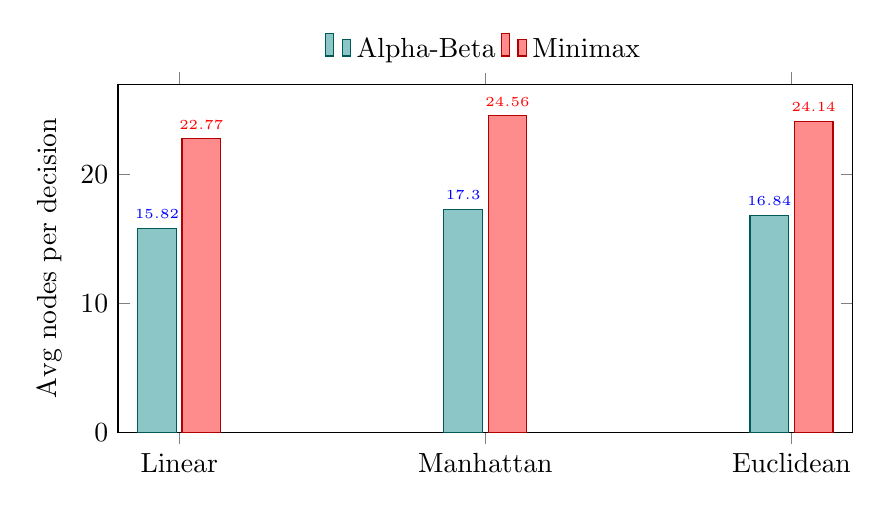
\begin{tikzpicture}
\begin{axis}[
    ybar,
    bar width=14pt,
    width=0.9\linewidth,
    height=6.0cm,
    ymin=0,
    ylabel={Avg nodes per decision},
    symbolic x coords={Linear,Manhattan,Euclidean},
    xtick=data,
    legend style={at={(0.5,1.03)}, anchor=south, legend columns=2, draw=none},
    nodes near coords,
    every node near coord/.append style={font=\tiny}
]
\addplot+[fill=teal!45, draw=teal!70!black] coordinates {
    (Linear,15.82)
    (Manhattan,17.297)
    (Euclidean,16.842)
};
\addplot+[fill=red!45, draw=red!70!black] coordinates {
    (Linear,22.767)
    (Manhattan,24.555)
    (Euclidean,24.139)
};
\legend{Alpha-Beta,Minimax}
\end{axis}
\end{tikzpicture}
\caption{Average expanded nodes by heuristic: Minimax vs Alpha-Beta.}
\label{fig:bars-nodes-by-heuristic}
\end{figure}

\begin{figure}[!htbp]
\centering
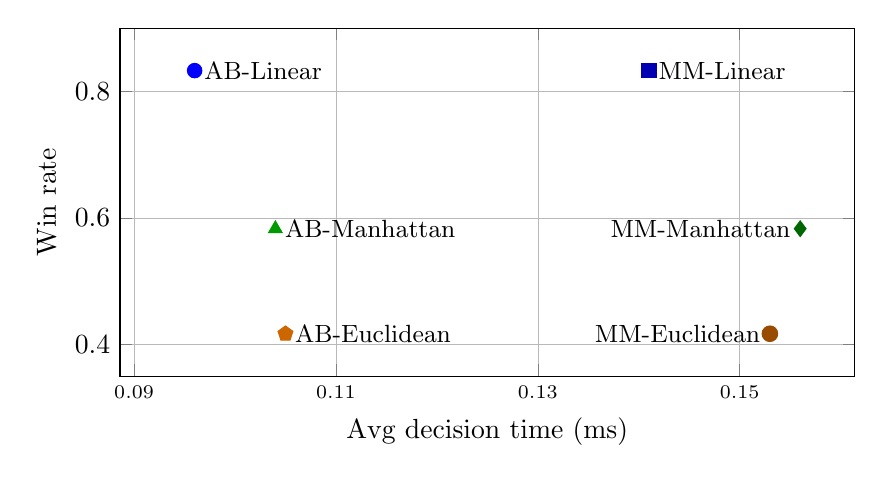
\begin{tikzpicture}
\begin{axis}[
    width=0.9\linewidth,
    height=6.0cm,
    xlabel={Avg decision time (ms)},
    ylabel={Win rate},
    xmin=0.09,
    xmax=0.16,
    ymin=0.35,
    ymax=0.9,
    enlarge x limits=0.02,
    scaled x ticks=false,
    xtick={0.09,0.11,0.13,0.15},
    xticklabel style={/pgf/number format/fixed,/pgf/number format/precision=2,font=\scriptsize},
    grid=both,
    grid style={line width=.1pt, draw=gray!30},
    major grid style={line width=.2pt, draw=gray!55}
]
\addplot[only marks, mark=*, mark size=2.6pt, blue] coordinates {(0.096,0.833)};
\addplot[only marks, mark=square*, mark size=2.6pt, blue!70!black] coordinates {(0.141,0.833)};
\addplot[only marks, mark=triangle*, mark size=2.8pt, green!60!black] coordinates {(0.104,0.583)};
\addplot[only marks, mark=diamond*, mark size=2.8pt, green!40!black] coordinates {(0.156,0.583)};
\addplot[only marks, mark=pentagon*, mark size=2.8pt, orange!80!black] coordinates {(0.105,0.417)};
\addplot[only marks, mark=otimes*, mark size=2.8pt, orange!60!black] coordinates {(0.153,0.417)};

\node[anchor=west, font=\small] at (axis cs:0.096,0.833) {AB-Linear};
\node[anchor=west, font=\small] at (axis cs:0.141,0.833) {MM-Linear};
\node[anchor=west, font=\small] at (axis cs:0.104,0.583) {AB-Manhattan};
\node[anchor=east, font=\small] at (axis cs:0.156,0.583) {MM-Manhattan};
\node[anchor=west, font=\small] at (axis cs:0.105,0.417) {AB-Euclidean};
\node[anchor=east, font=\small] at (axis cs:0.153,0.417) {MM-Euclidean};
\end{axis}
\end{tikzpicture}
\caption{Efficiency vs quality: average decision time against win rate.}
\label{fig:scatter-efficiency-quality}
\end{figure}
\FloatBarrier

\subsection{Discussion}
Los resultados arrojados en el torneo se muestran en las Tablas \ref{tab:summary-main} y \ref{tab:summary-outcomes-ci}. En términos de 
desempeño competitivo entre algoritmos, se evidencia que la heurística más efectiva fue la \textit{lineal}, presentando 10 victorias, 1 derrota y 1 empate; en segundo lugar, se establece la heurística Manhattan con 7 victorias, 5 derrotas y 0 empates, seguida por la heurística euclidiana con 5 victorias, 7 derrotas y 0 empates. Para respaldar esa tendencia, la diferencia promedio de puntos sigue un comportamiento similar, en el cual \textit{lineal} presenta un margen
positivo de 5.583, Manhattan un margen casi neutro de -0.333 y Euclediana un margen negativo de -3.667.\\

Esta clara superioridad de la heurística lineal no es accidental; ocurre porque su evaluación multidimensional captura el comportamiento real del dominó
con más precisión, ya que tiene en cuenta \textbf{4 características del estado del juego}: la cantidad de fichas, los puntos, la movilidad del jugador y el control sobre los extremos de la mesa. Mientras que Manhattan y Euclediana, al ser aproximaciones espaciales, intentan simplificar la asimilación del juego al enfocarse casi exclusivamente en reducir el valor acumulado (puntos), perdiendo de vista las otras características fundamentales del dominó, como bloquear los extremos del tablero o evaluar la movilidad del jugador (opciones de juego), que, como ya se mencionó, lineal sí tiene en cuenta.\\

Con respecto al costo computacional, la Figura \ref{fig:bars-nodes-by-heuristic} y la Figura \ref{fig:scatter-efficiency-quality} exponen el profundo impacto de la arquitectura de búsqueda implementada. Se observa que, independientemente de la métrica de éxito (win rate, victorias o diferencia de puntos), los algoritmos Minimax, tanto con poda Alfa-Beta como sin esta, obtuvieron resultados exactos bajo la misma profundidad de exploración (\textit{depth = 3}). Este fenómeno demuestra la base teórica de la poda Alpha-Beta: al acotar iterativamente el árbol de contingencias de jugadas, el algoritmo logra descartar de manera efectiva ramificaciones del árbol inútiles, reduciendo alrededor del 30\% de los nodos evaluados sin alterar la efectividad del enfoque estándar de "fuerza bruta" que tiene Minimax.\\

Como resultado de esta menor tasa de evaluación de estados, la poda Alpha-Beta fue drásticamente más eficiente. Este algoritmo reduce en un rango del 31\% al 33\% el tiempo promedio computacional por decisión frente al Minimax crudo, reduciendo consecuentemente los picos de máxima latencia durante jugadas más difusas. Esta mitigación de latencia o consumo en tiempo es uno de los mayores logros del agente, puesto que alude a la capacidad de obviar ramas enteras del árbol sin sacrificar el resultado final, generando una compensación  (\textit{trade-off}), ya que al utilizar una ventana de tiempo predefinida (\textit{time budget}) equivalente a la que usaría el algoritmo sin optimizar,  le permitiría a la versión con Alpha-Beta sumergirse y examinar el juego a mayores profundidades (\textit{depth} $>$ 3), optimizando el rendimiento estratégico y reduciendo la incertidumbre en un entorno en tiempo real. La poda Alfa-Beta tal vez no mejoró la cantidad de victorias por la profundidad limitada, pero presenta un inmenso potencial para escalar.\\

Finalmente, aunque los resultados comprueban que el conjunto emparejado de \textit{Minimax}, \textit{poda Alpha-Beta} y \textit{heurística Lineal} confiere el nivel más alto de precisión y rentabilidad del benchmark, se reconocen los límites en esta versión del modelo. Al tratarse de un experimento limitado al escopo de exploración de tres niveles de profundidad contra un rival predefinido \textit{Greedy}, el entorno de demostración se mantiene algo sesgado frente a la inmensurable variedad del juego. Como trabajo próximo queda estipular cuán eficiente es dicho agente si el presupuesto de exploración aumenta en iteraciones dinámicas o si el rival está dotado de estrategias estocásticas y/o enfoques de red neuronal.


\section{Conclusion}
En esta investigación se diseñó e implementó exitosamente un agente inteligente capaz de competir en el juego de dominó, demostrando el impacto directo que tiene el diseño de la función heurística
y la optimización de los algoritmos de búsqueda adversarial en la eficiencia computacional y el desempeño táctico. Los resultados comprobaron empíricamente que la técnica de poda Alfa-Beta y el algoritmo 
Minimax base producen decisiones idénticas bajo la misma cota de exploración, pero la poda Alfa-Beta optimiza el rendimiento general reduciendo aproximadamente en un 33\% la latencia de respuesta y 
en un 30\% el tamaño del árbol de nodos explorados. Por otro lado, al evaluar los métodos para puntuar los estados del juego, la heurística espacial (Manhattan y Euclidiana) mostró severas limitantes 
al abstraer el entorno puramente hacia el descarte del valor total en la mano; mientras que la heurística Lineal —al incorporar múltiples dimensiones como la movilidad, la cantidad de fichas, y fundamentalmente, e
l control del tablero— otorgó un dominio sustancial de las partidas, logrando una tasa de victoria protagónica. En síntesis, la conjunción de Minimax, poda Alfa-Beta y heurística Lineal estructuró un modelo óptimo, 
dotando al agente de un razonamiento estratégico robusto bajo tiempos de respuesta computacionalmente viables.


\section{Future Work}
A partir de las limitantes identificadas en el entorno experimental actual y la naturaleza heurística del agente, se proponen las siguientes líneas de trabajo para la optimización y escalabilidad del proyecto en un futuro:
\begin{itemize}
    \item \textbf{Aumento dinámico de la profundidad de exploración:} Implementar técnicas como \textit{Iterative Deepening} en sincronía con la 
    poda Alfa-Beta, buscando aprovechar íntegramente el presupuesto de tiempo (\textit{time budget}) ahorrado. Esto permitiría al agente profundizar
    asimétricamente en las rutas más prometedoras, rompiendo la barrera estática planteada en los tests (\textit{depth = 3}).
    \item \textbf{Inferencia probabilística de la mano rival:} Transicionar hacia un modelo que aproveche el historial de la mesa. 
    Al incorporar estructuras de conteo de fichas caídas, el agente podría deducir probabilísticamente la mano del adversario, refinando la 
    heurística para adaptarse a un entorno con información oculta asimilando el comportamiento analítico humano.
    \item \textbf{Competencia contra arquitecturas neuro-estocásticas:} Someter al modelo a torneos sistemáticos frente a agentes oponentes 
    dotados por algoritmos alternativos como árboles de búsqueda de Monte Carlo (MCTS) o redes neuronales entrenadas por Aprendizaje por Refuerzo,
    lo que proveerá una validación comparativa ante la incertidumbre que supera a las validaciones aisladas frente a un modelo \textit{Greedy}.
    \item \textbf{Escalabilidad de entorno cooperativo:} Expandir la lógica del agente y la parametrización minimax 
    (adaptando enfoques como \textit{Max\textsuperscript{N}}) para abarcar la modalidad por parejas (2 vs 2), la cual es la estructura 
    competitiva más frecuente en el mundo, en donde las decisiones y heurísticas asuman no solo el propio beneficio y castigo enemigo,
    sino la sincronización y asistencia indirecta a un aliado.
\end{itemize}

\appendices
\section{Proof of the First Zonklar Equation}
Appendix one text goes here.

\section{}
Appendix two text goes here.




\bibliographystyle{IEEEtran}
\bibliography{referencias}

\end{document}


